
\subsection{Single Lepton Top MC Modelling Validation from CR2}
\label{sec:cr2}


The \mt\ tail for single-lepton top events (\ttsl\ and single top) is dominated by jet resolution effects. The \W\ cannot be far off-shell because $\mW < \mtop$.
The modeling of the \mt\ tail from jet resolution effects is studied
using \zjets\ data and MC samples. 

\Z\ events are selected by requiring exactly 2 good leptons (satisfying ID
and isolation requirements) and requiring the \mll\ to be in the range
$81-101$ GeV. 
Events with additional isolated tracks are vetoed, as in Section~\ref{sec:tkveto}.
To reduce \ttbar\ backgrounds, events with a CSVM tag %H
are removed.
The negative lepton is treated as a neutrino and so is added to the MET: \met\ $\rightarrow$ \pt(\Lepm) + \met, 
and the \mt\ is recalculated with the positive lepton \mt(\Lepp, \met).
The resulting ``pseudo-\mt'' is dominated by jet resolution effects, since no off-shell 
\Z\ production enters the sample due to the \mll\ requirement.
This section describes how well the MC predicts the tail of ``pseudo-\mt''. 

The underlying distributions are shown in Fig.~\ref{fig:cr2met}
and~\ref{fig:cr2mtrest}.    Just as in CR1, there is an excess in the
tails, but there are insufficient events to derive scale factors.
% for $\met\ > 150$~GeV.


%We then perform the exact same type of Data/MC comparison and analysis as 
%described for CR1 in Section~\ref{sec:cr1}.  For CR1 we collected
%the data/MC tail information in 
%Table~\ref{tab:cr1yields} ; the equivalent for CR2 is
%Table~\ref{tab:cr2yields}
%(for CR2 the statistics are not sufficient to split electrons and muons).
%The last line of Table~\ref{tab:cr2yields} gives the data/MC scale factor
%for the \ttbar\ lepton $+$ jets $M_T$ tail ($SFR_{top}$).  This is
%calculated in the same way as $SFR_{wjets}$ of Table~\ref{tab:cr1yields}.


\begin{table}[!h]
\begin{center}
{\footnotesize
\begin{tabular}{l||c|c||c|c|c|c|c}
\hline
Sample              & CR2PRESEL0 &CR2PRESEL1 & CR2A & CR2B & CR2C &
CR2D & CR2E \\
\hline
\hline
MC 		  & $36 \pm 2$ & $30 \pm 2$ & $18 \pm 1$ & $30 \pm 2$ & $13 \pm 1$ & $5 \pm 0$ & $2 \pm 0$ \\
Data 		  & $56$ & $43$ & $32$ & $40$ & $21$ & $12$ & $2$ \\
\hline
Data/MC 	  & $1.56 \pm 0.23$ & $1.44 \pm 0.24$ & $1.77 \pm 0.34$ & $1.32 \pm 0.22$ & $1.65 \pm 0.37$ & $2.65 \pm 0.79$ & $0.99 \pm 0.71$ \\
\hline
\hline
\hline
DY MC 		  & $27 \pm 2$ & $23 \pm 2$ & $14 \pm 2$ & $25 \pm 3$ & $11 \pm 2$ & $3 \pm 1$ & $1 \pm 1$ \\
DY Data 	  & $47 \pm 8$ & $36 \pm 7$ & $28 \pm 6$ & $35 \pm 6$ & $19 \pm 5$ & $11 \pm 3$ & $1 \pm 1$ \\
\hline
DY Data/MC 	  & $1.75 \pm 0.31$ & $1.58 \pm 0.32$ & $2.00 \pm 0.47$ & $1.38 \pm 0.31$ & $1.78 \pm 0.56$ & $3.29 \pm 1.73$ & $0.98 \pm 1.20$ \\
\hline
\hline
\hline
$SFR_{top}$ 	  & $1.66 \pm 0.40$ & $1.51 \pm 0.35$ & $1.89 \pm 0.56$ & $1.35 \pm 0.28$ & $1.71 \pm 0.51$ & $2.97 \pm 1.26$ & $0.98 \pm 0.71$ \\
\hline
\end{tabular}}
\caption{ Yields in \mt\ tail comparing the \zjets\ MC prediction (after
  applying SFs) to data without subtracting the non-\zjets\ components (top table) and with subtracting the non-\zjets\ components (bottom table). 
  CR2PRESEL refers to a sample with $\met>50$ GeV and $\mt>150$ GeV.
\label{tab:cr2yields}}
\end{center}
\end{table}


\begin{figure}[hbt]
  \begin{center}
%	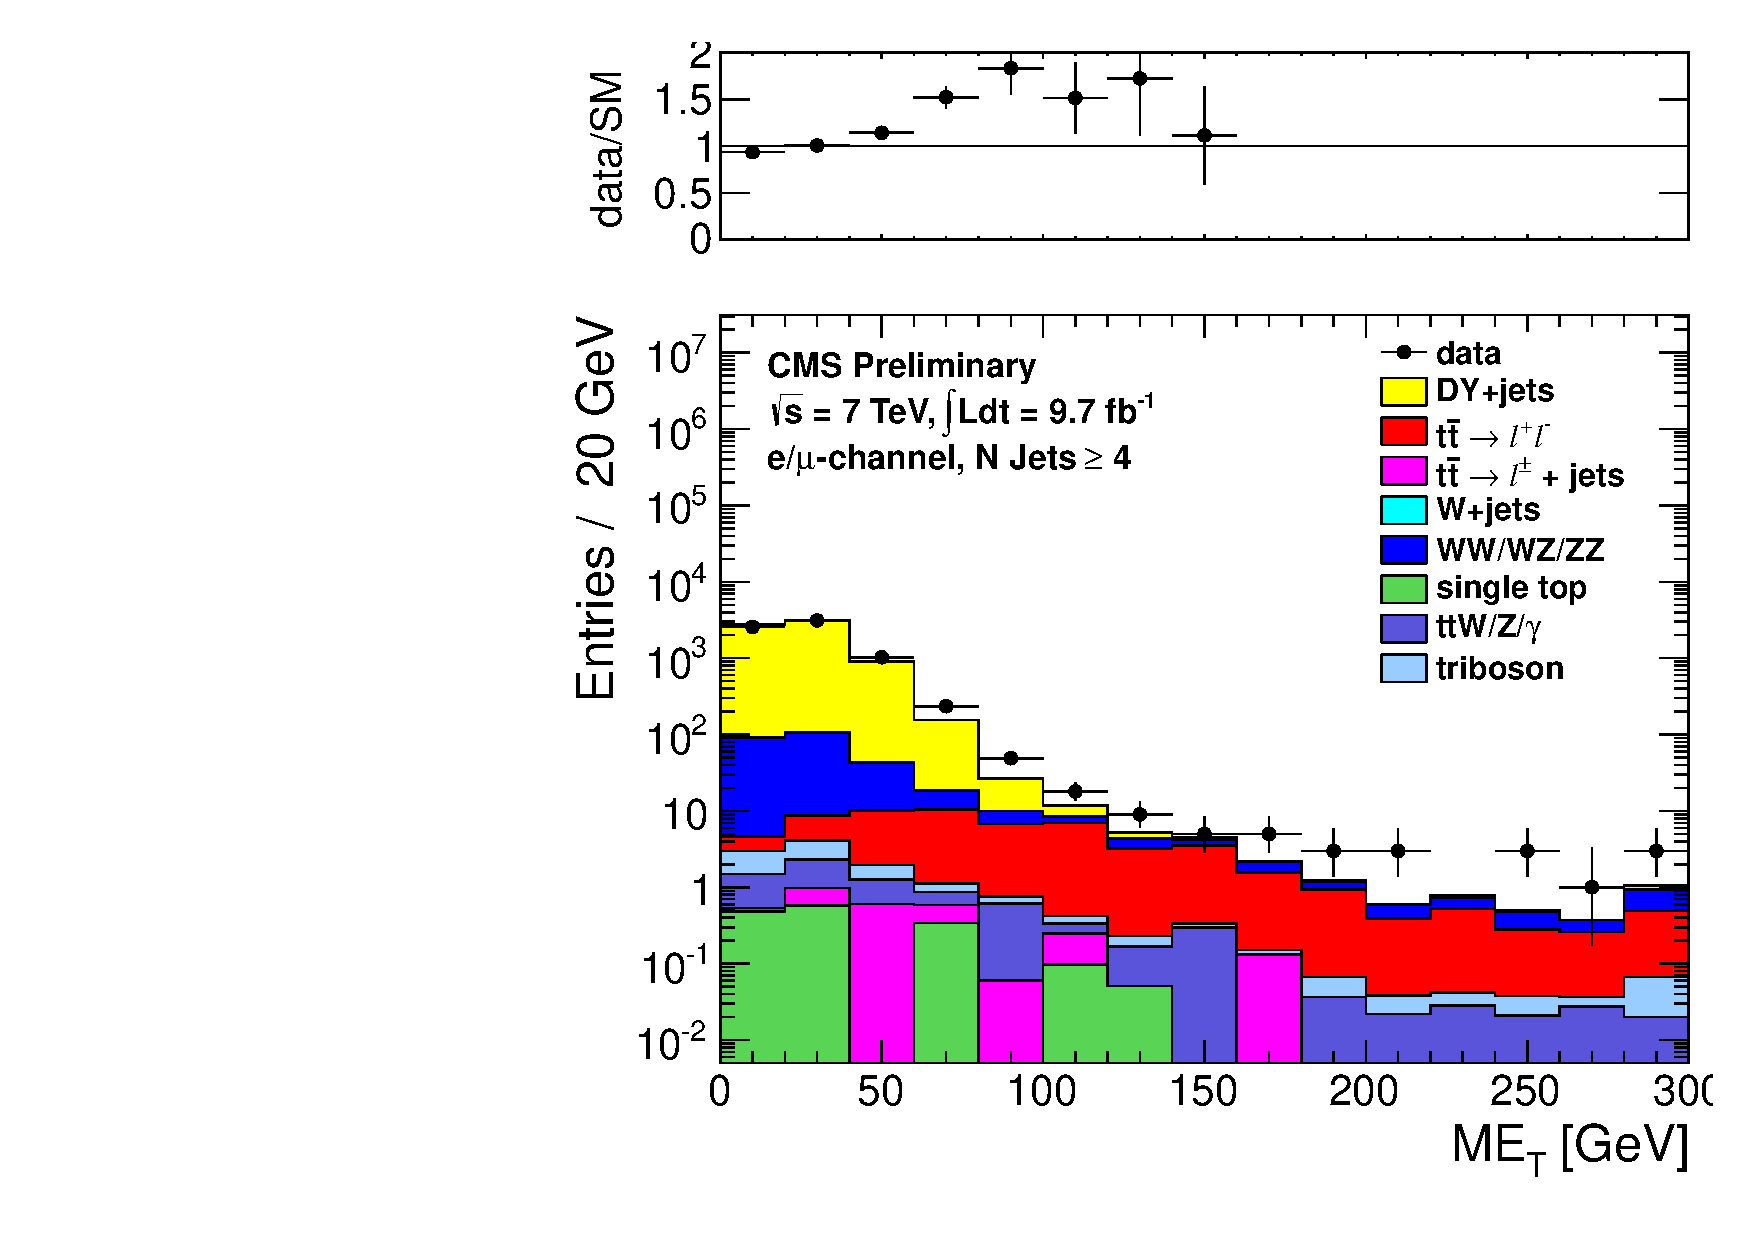
\includegraphics[width=0.5\linewidth]{plots/CR2plots/met_scaled_nj4_emucomb.pdf}%
	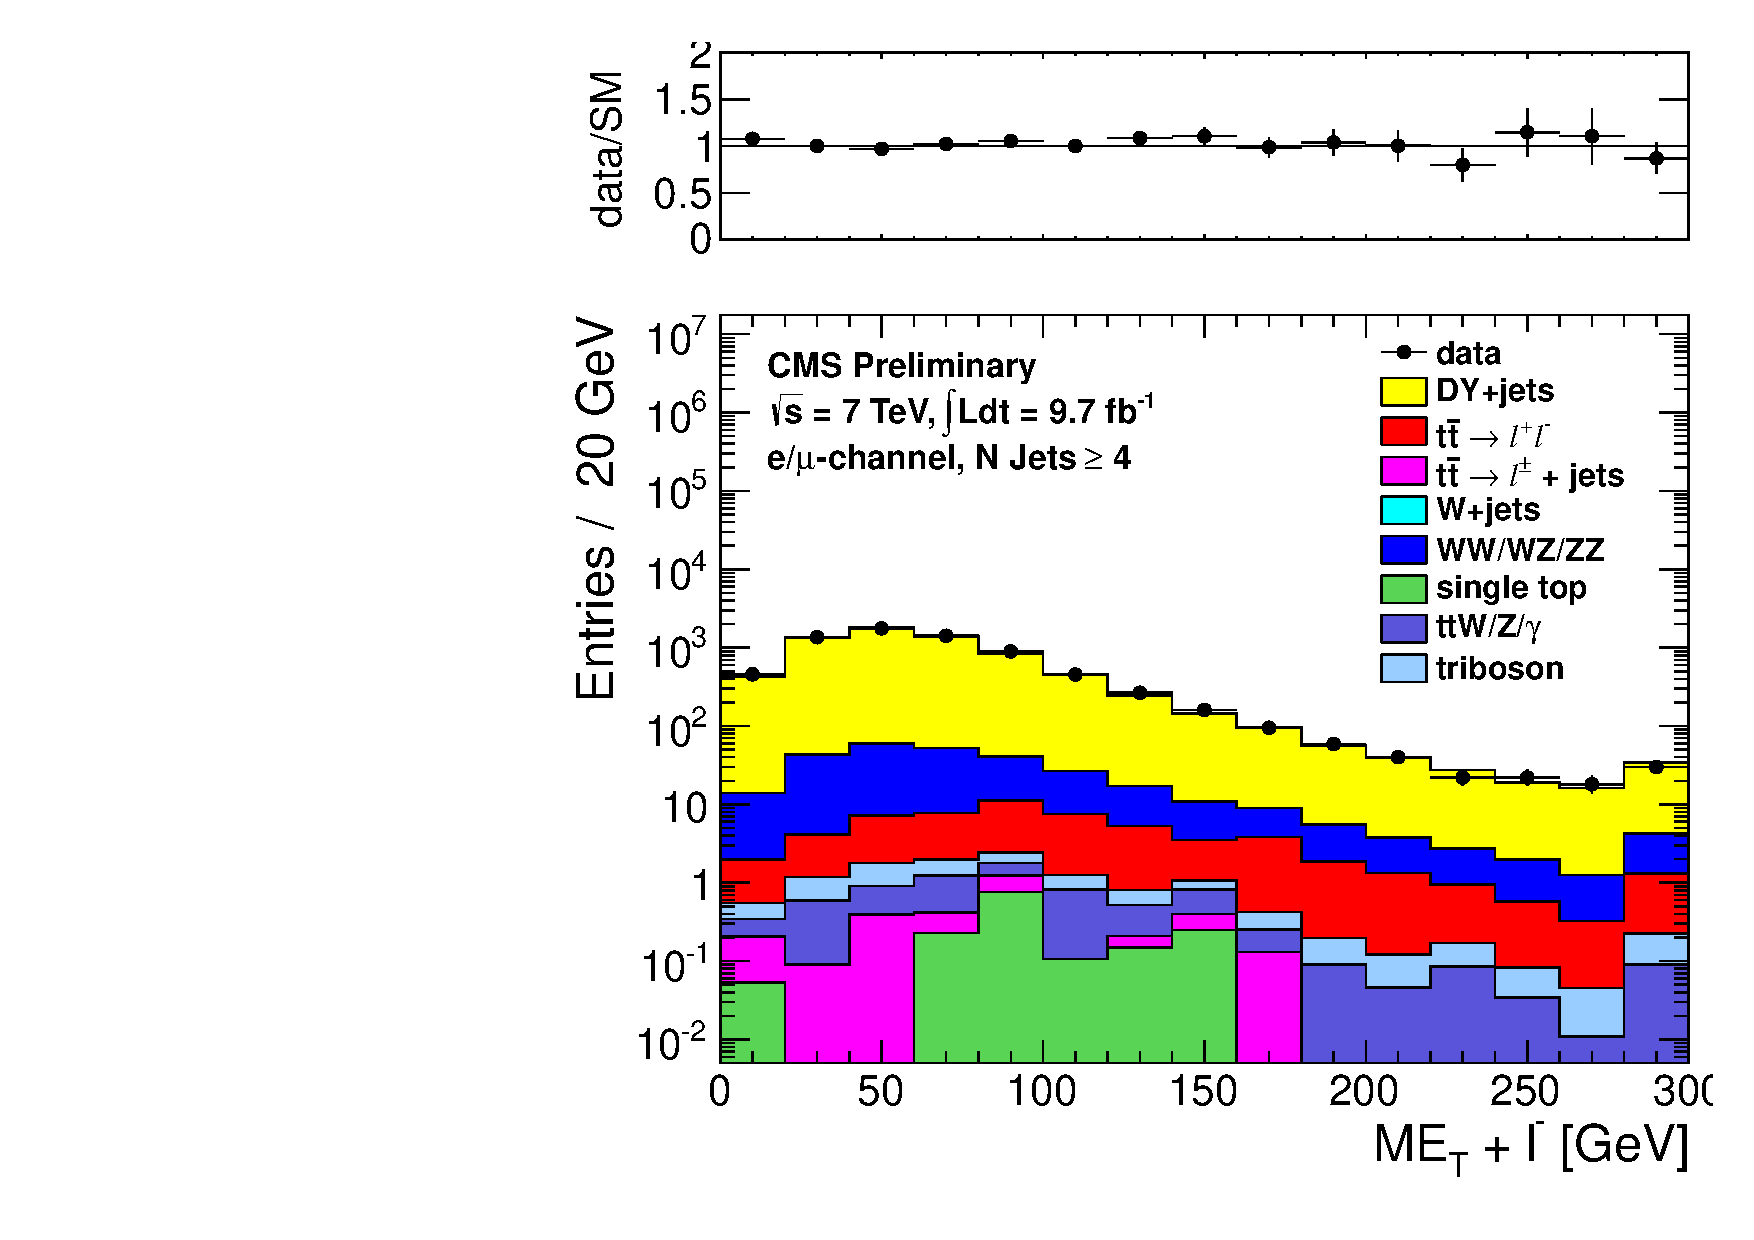
\includegraphics[width=0.5\linewidth]{plots/CR2plots/met_lepcor_scaled_nj4_emucomb.pdf}%
	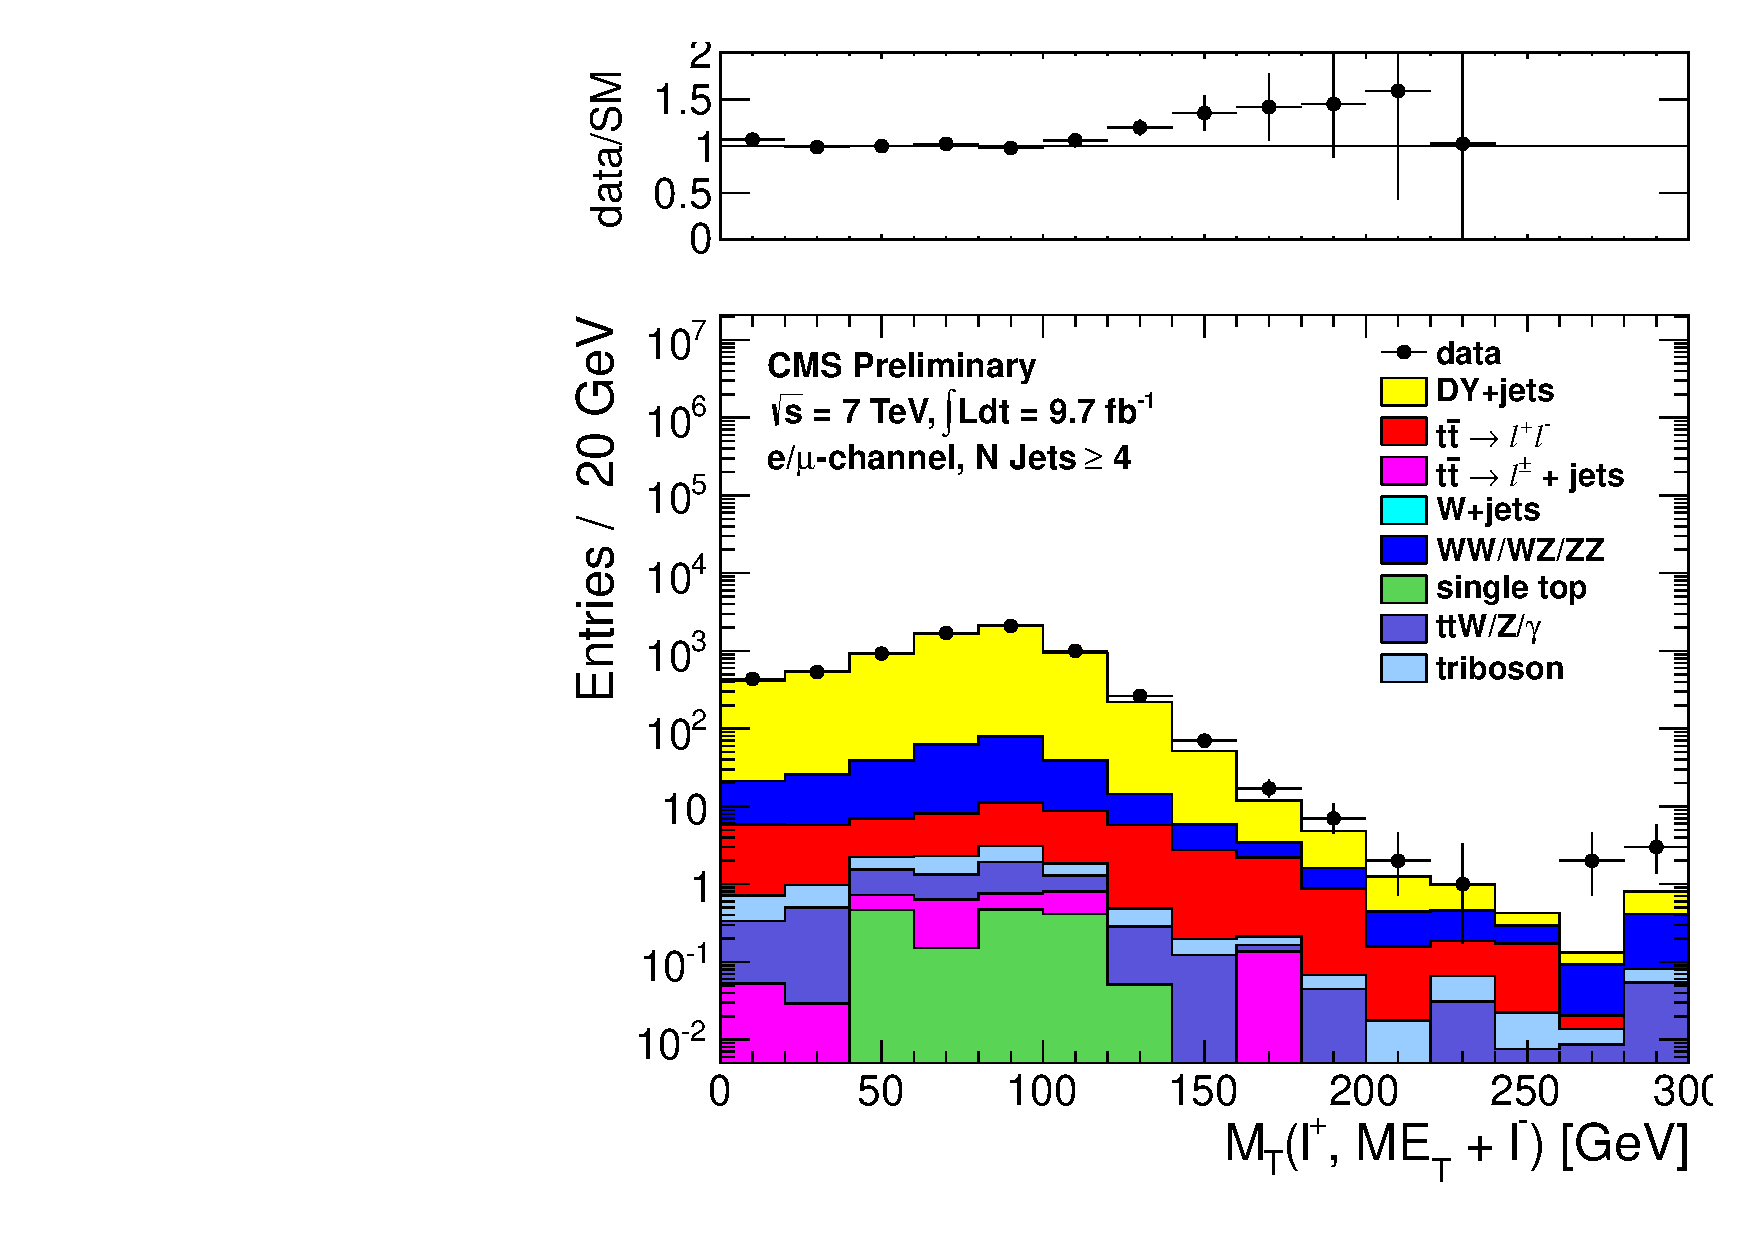
\includegraphics[width=0.5\linewidth]{plots/CR2plots/mt_lepcor_scaled_nj4_emucomb.pdf}
	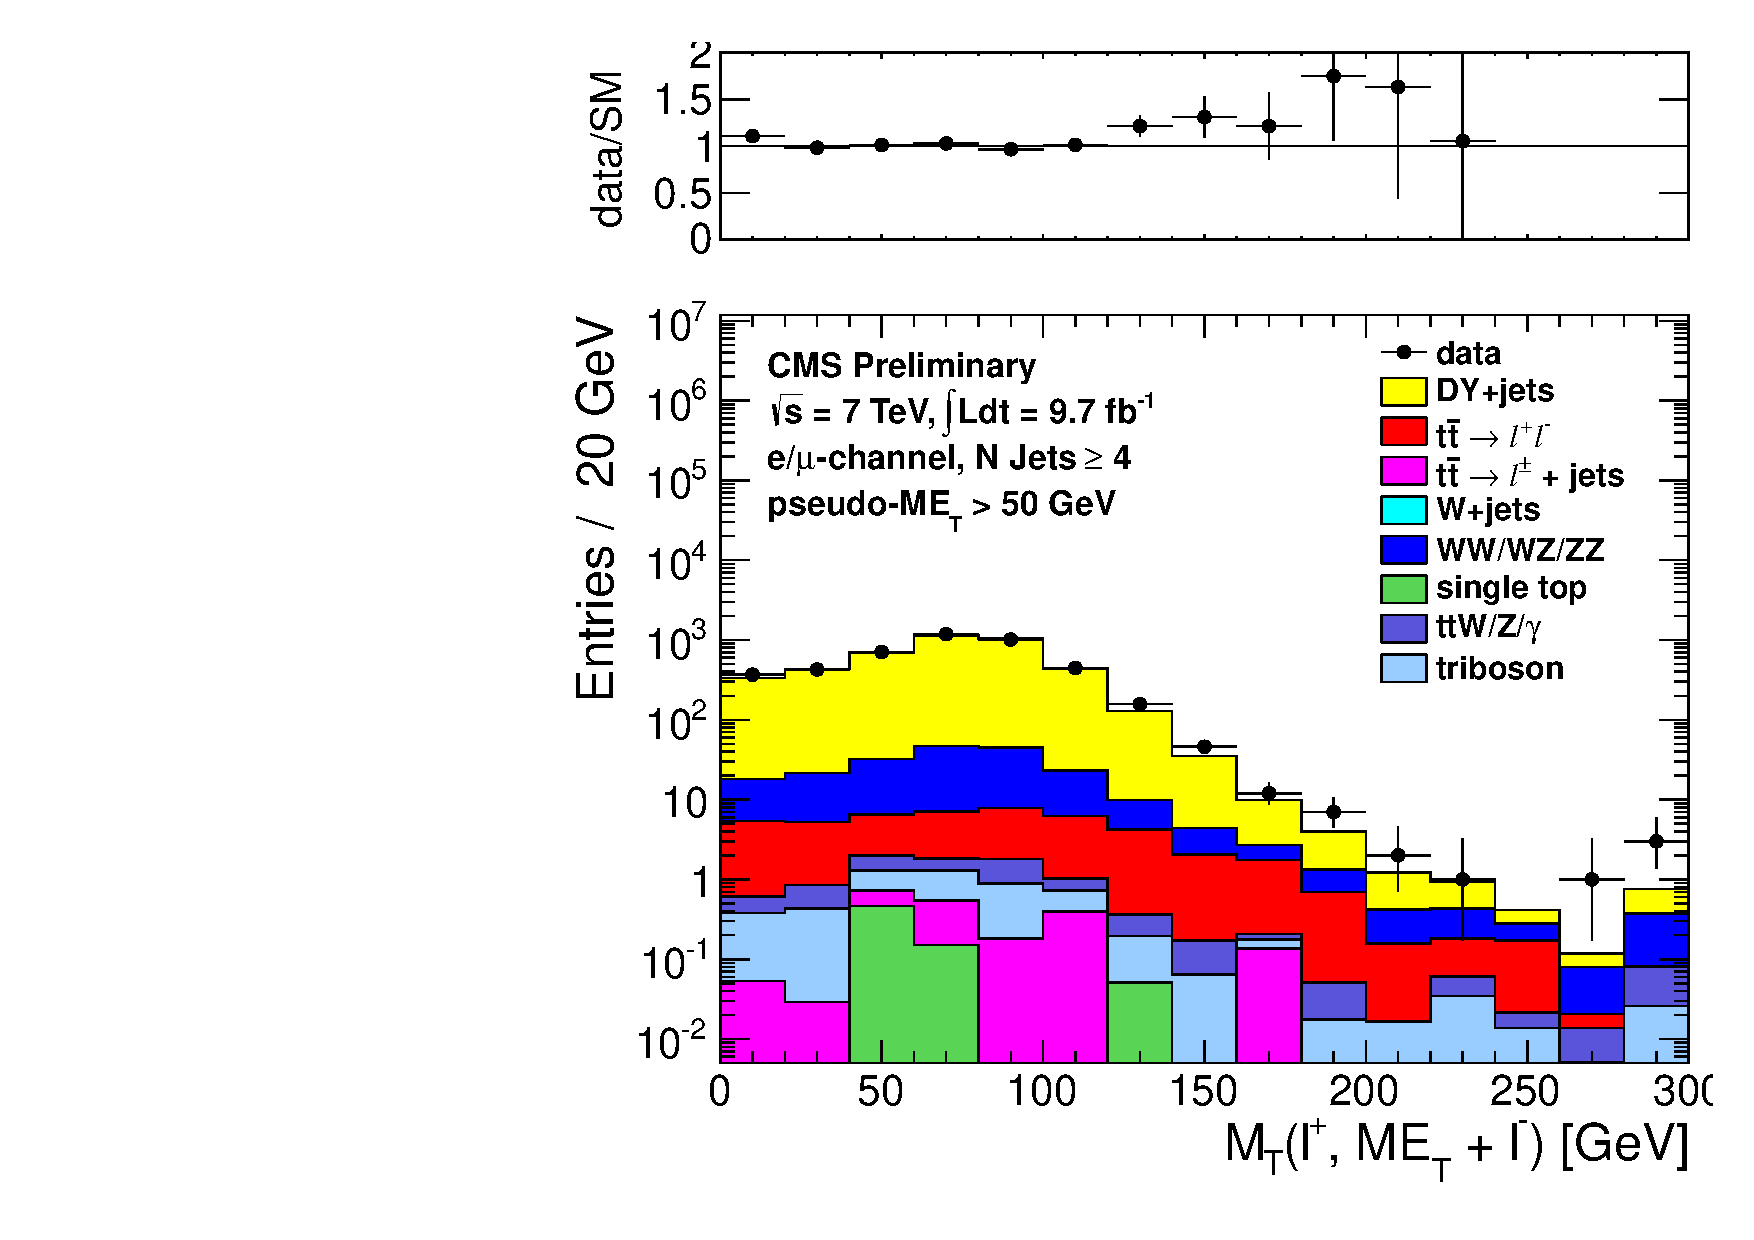
\includegraphics[width=0.5\linewidth]{plots/CR2plots/mt_lepcor_scaled_met50_nj4_emucomb.pdf}%
	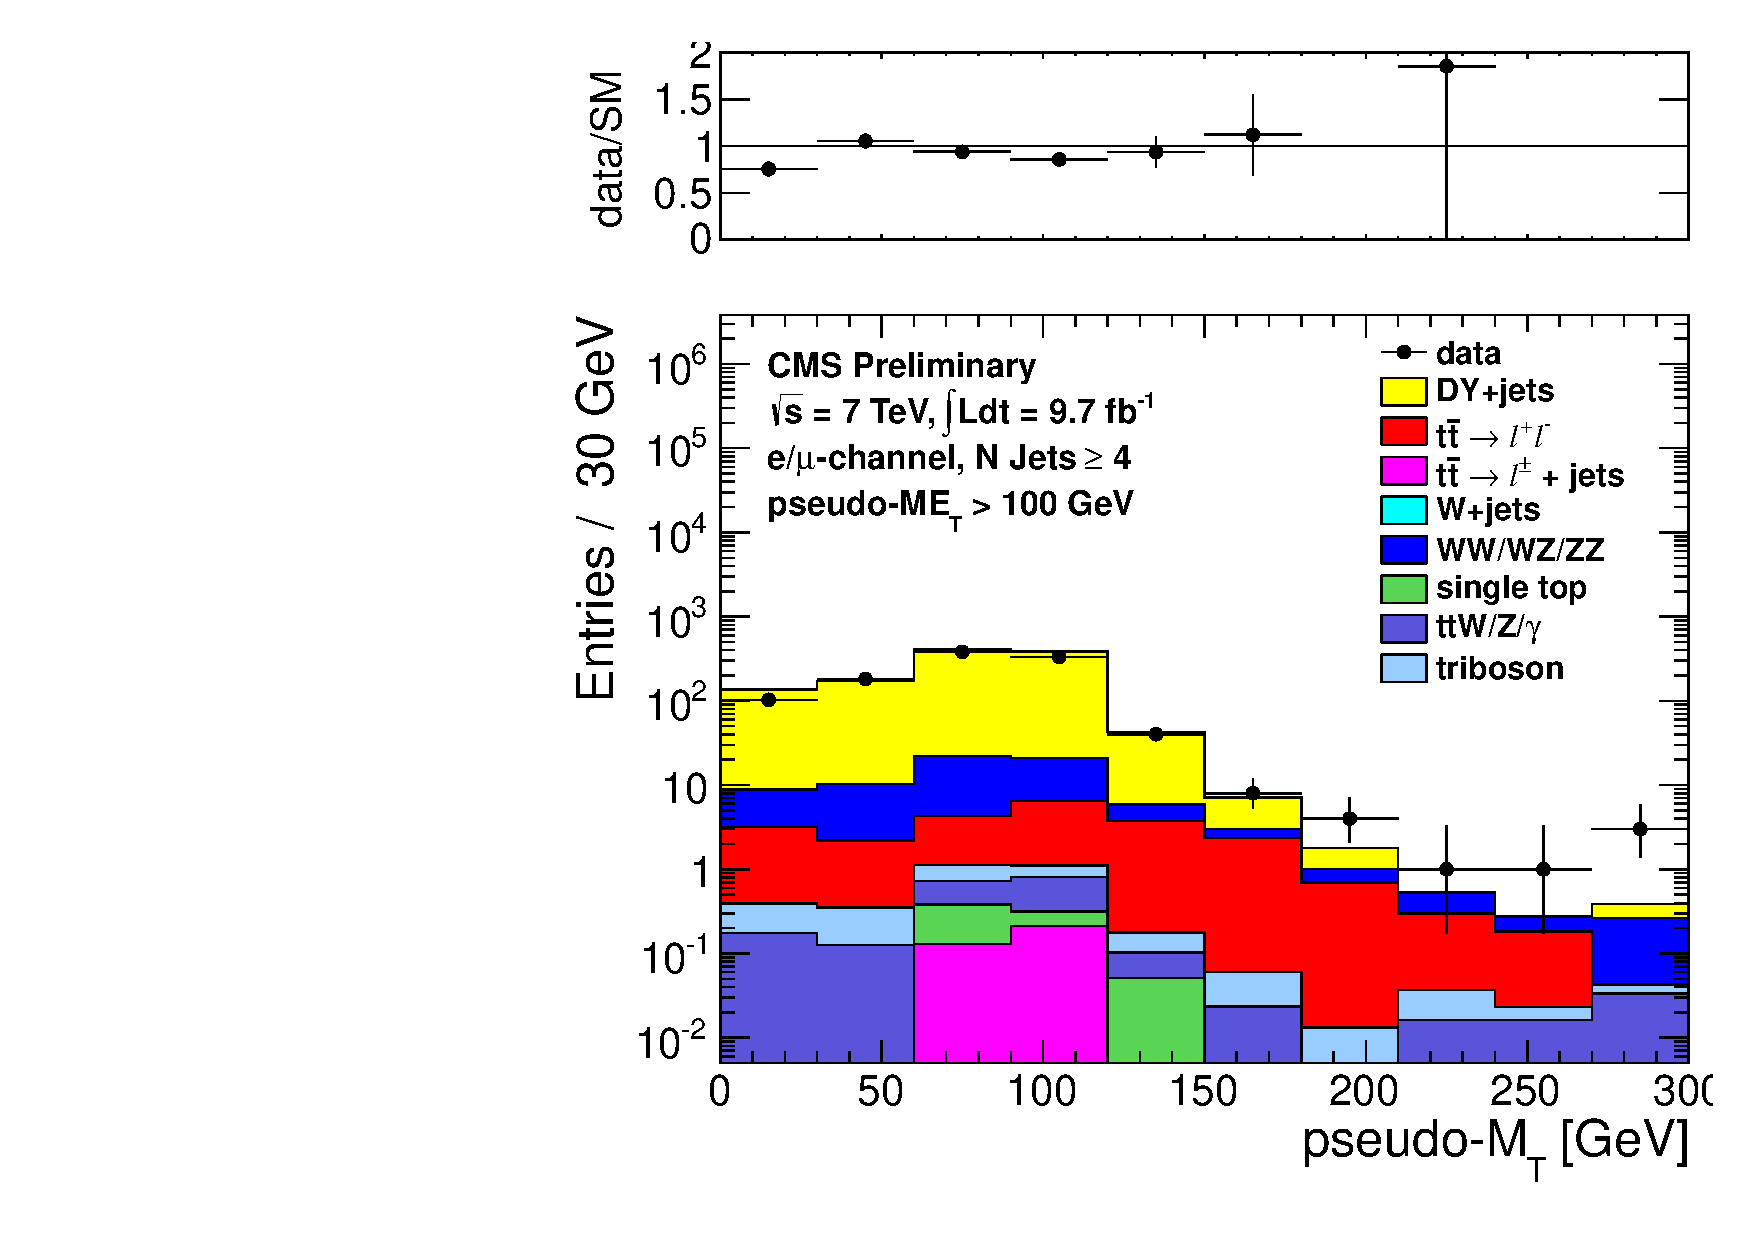
\includegraphics[width=0.5\linewidth]{plots/CR2plots/mt_lepcor_scaled_met100_nj4_emucomb.pdf}

    \caption{
      Comparison of the pseudo-\met\ (top, left), pseudo-\mt\ (top,
      right and bottom) distributions in data vs. MC for events
      satisfying the requirements of CR2, combining both the muon and
      electron channels. The pseudo-\mt\ distributions are shown
      before any additional requirements (top, right) and after
      requiring pseudo-\met $>$50 GeV (bottom, left) and pseudo-\met
      $>$ 100 GeV (bottom, right) .
\label{fig:cr2met} 
}  
      \end{center}
\end{figure}

\begin{figure}[hbt]
  \begin{center}
	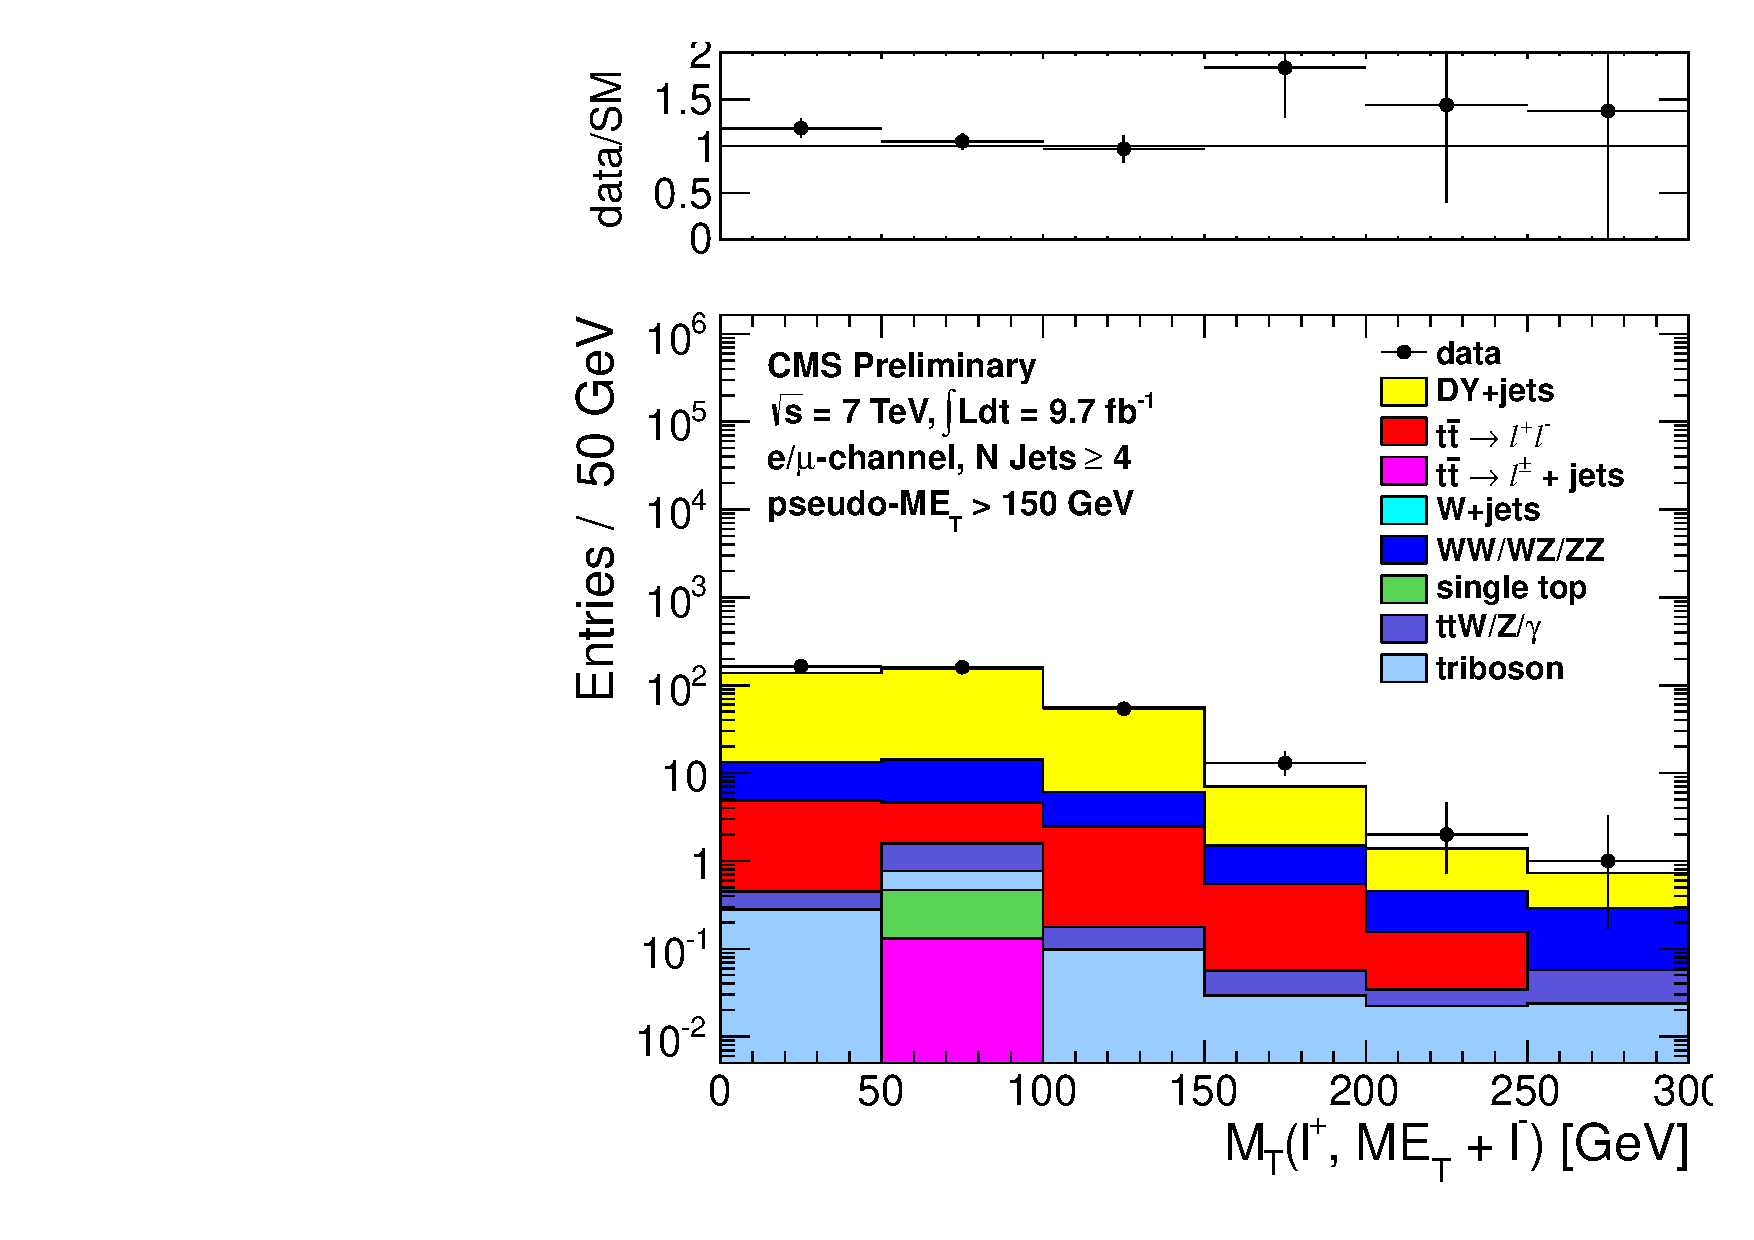
\includegraphics[width=0.5\linewidth]{plots/CR2plots/mt_lepcor_scaled_met150_nj4_emucomb.pdf}%
	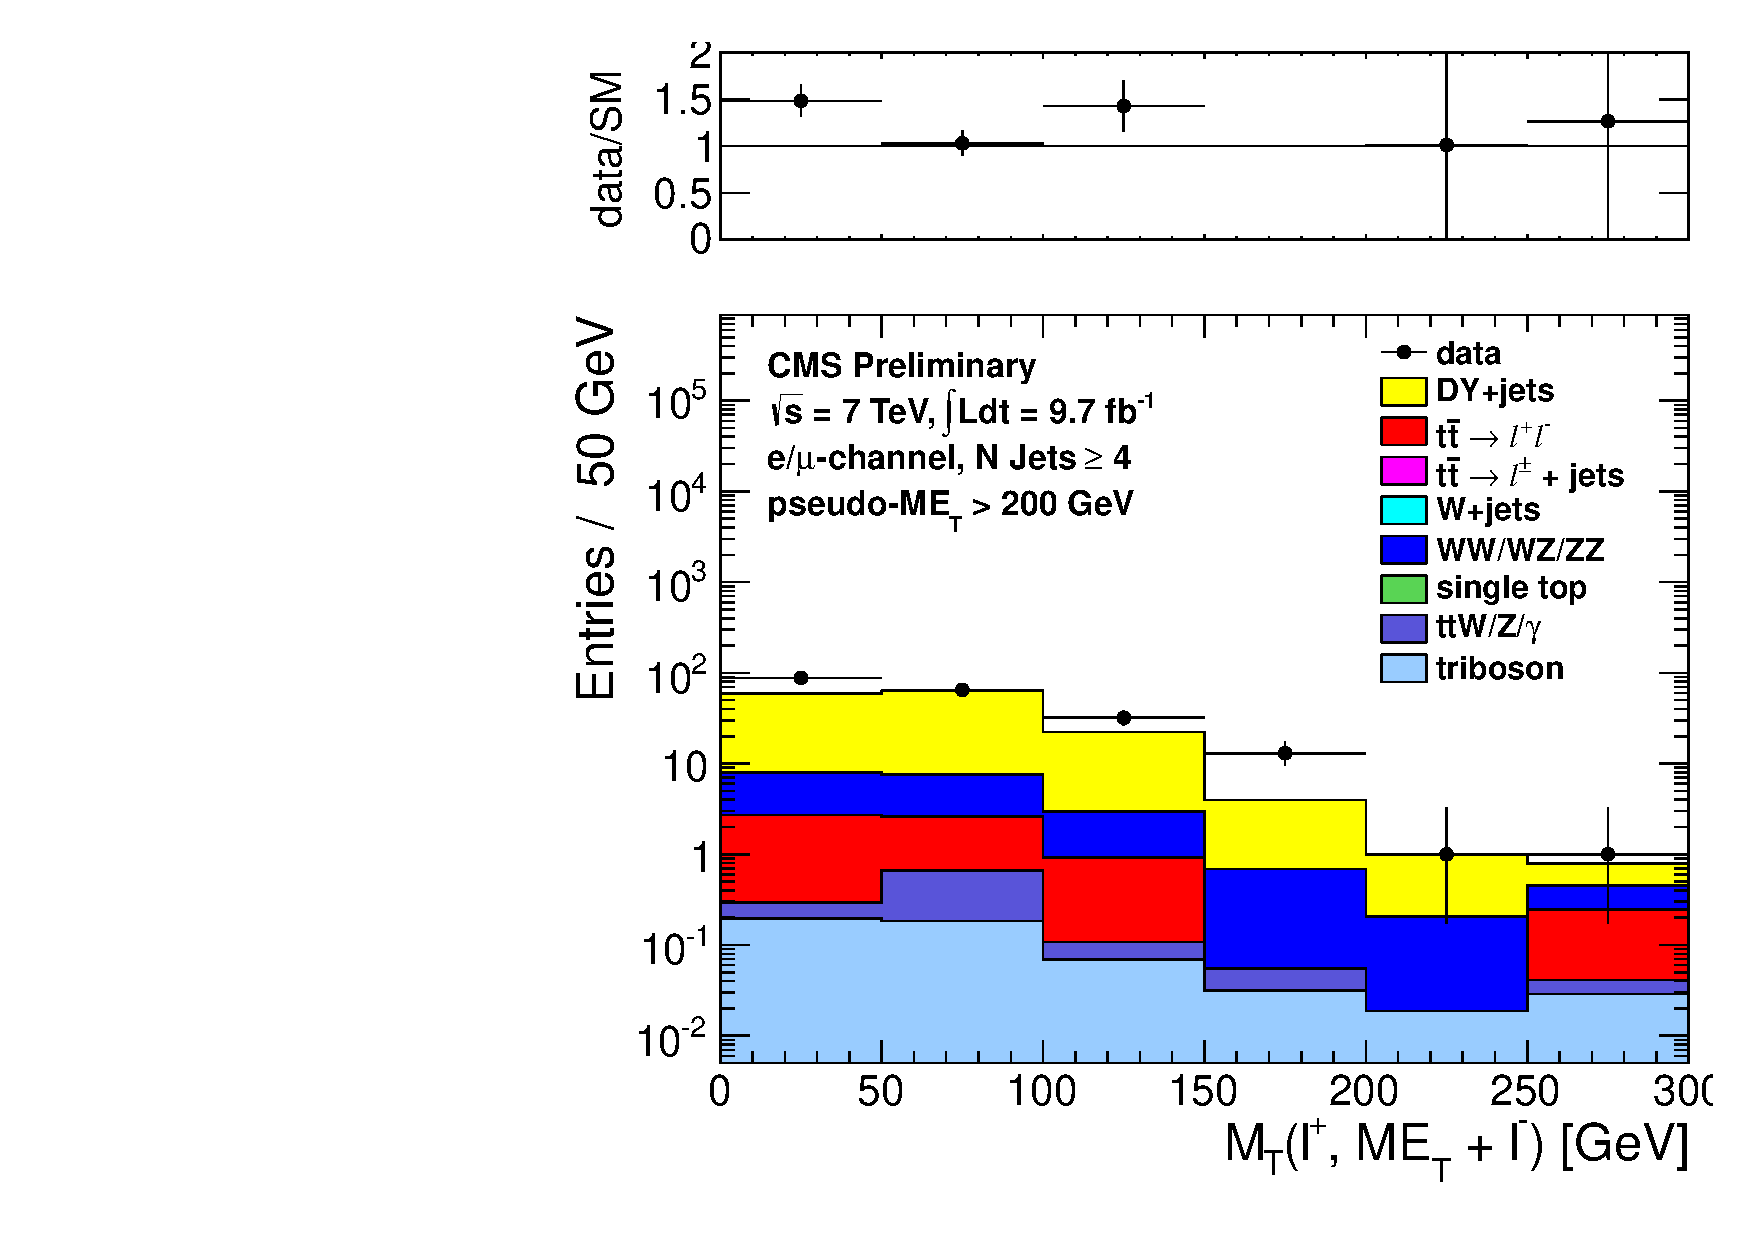
\includegraphics[width=0.5\linewidth]{plots/CR2plots/mt_lepcor_scaled_met200_nj4_emucomb.pdf}
	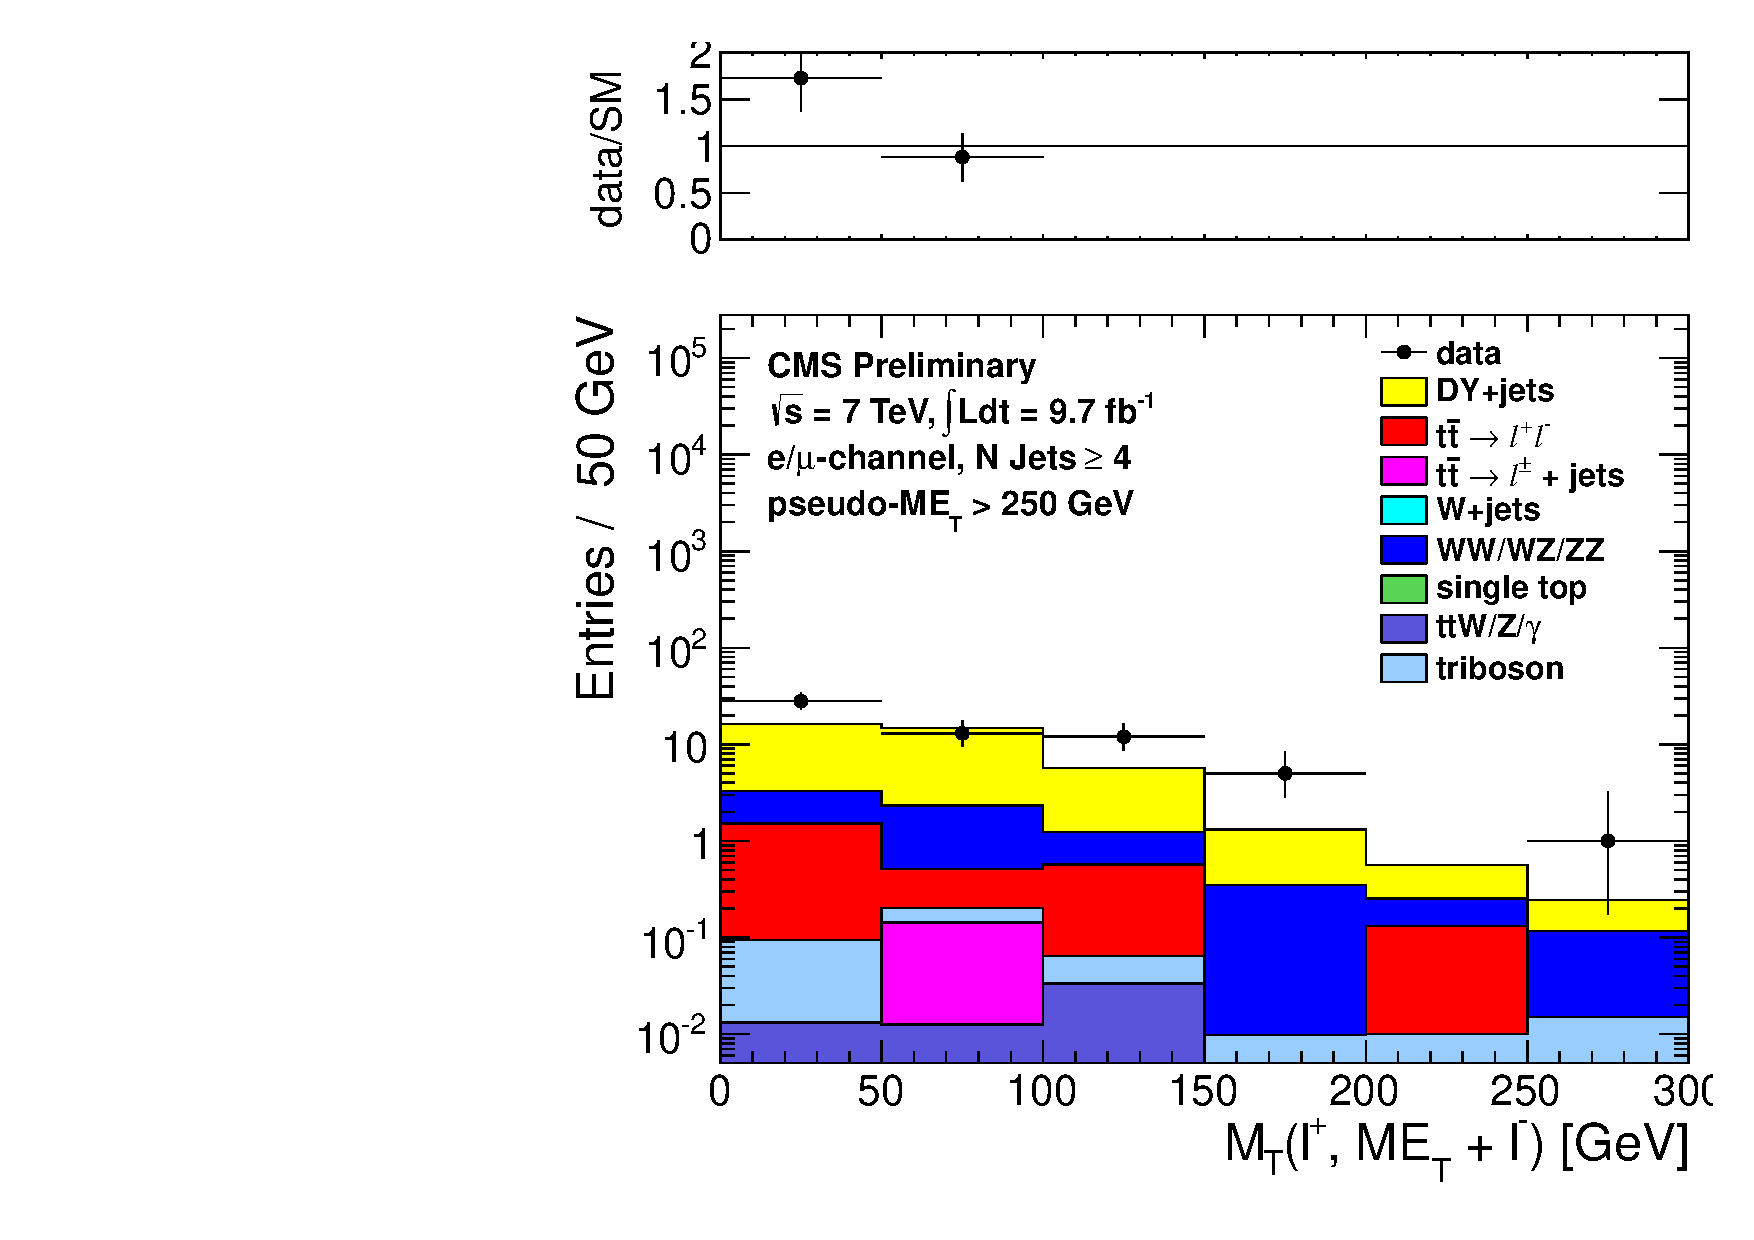
\includegraphics[width=0.5\linewidth]{plots/CR2plots/mt_lepcor_scaled_met250_nj4_emucomb.pdf}%
	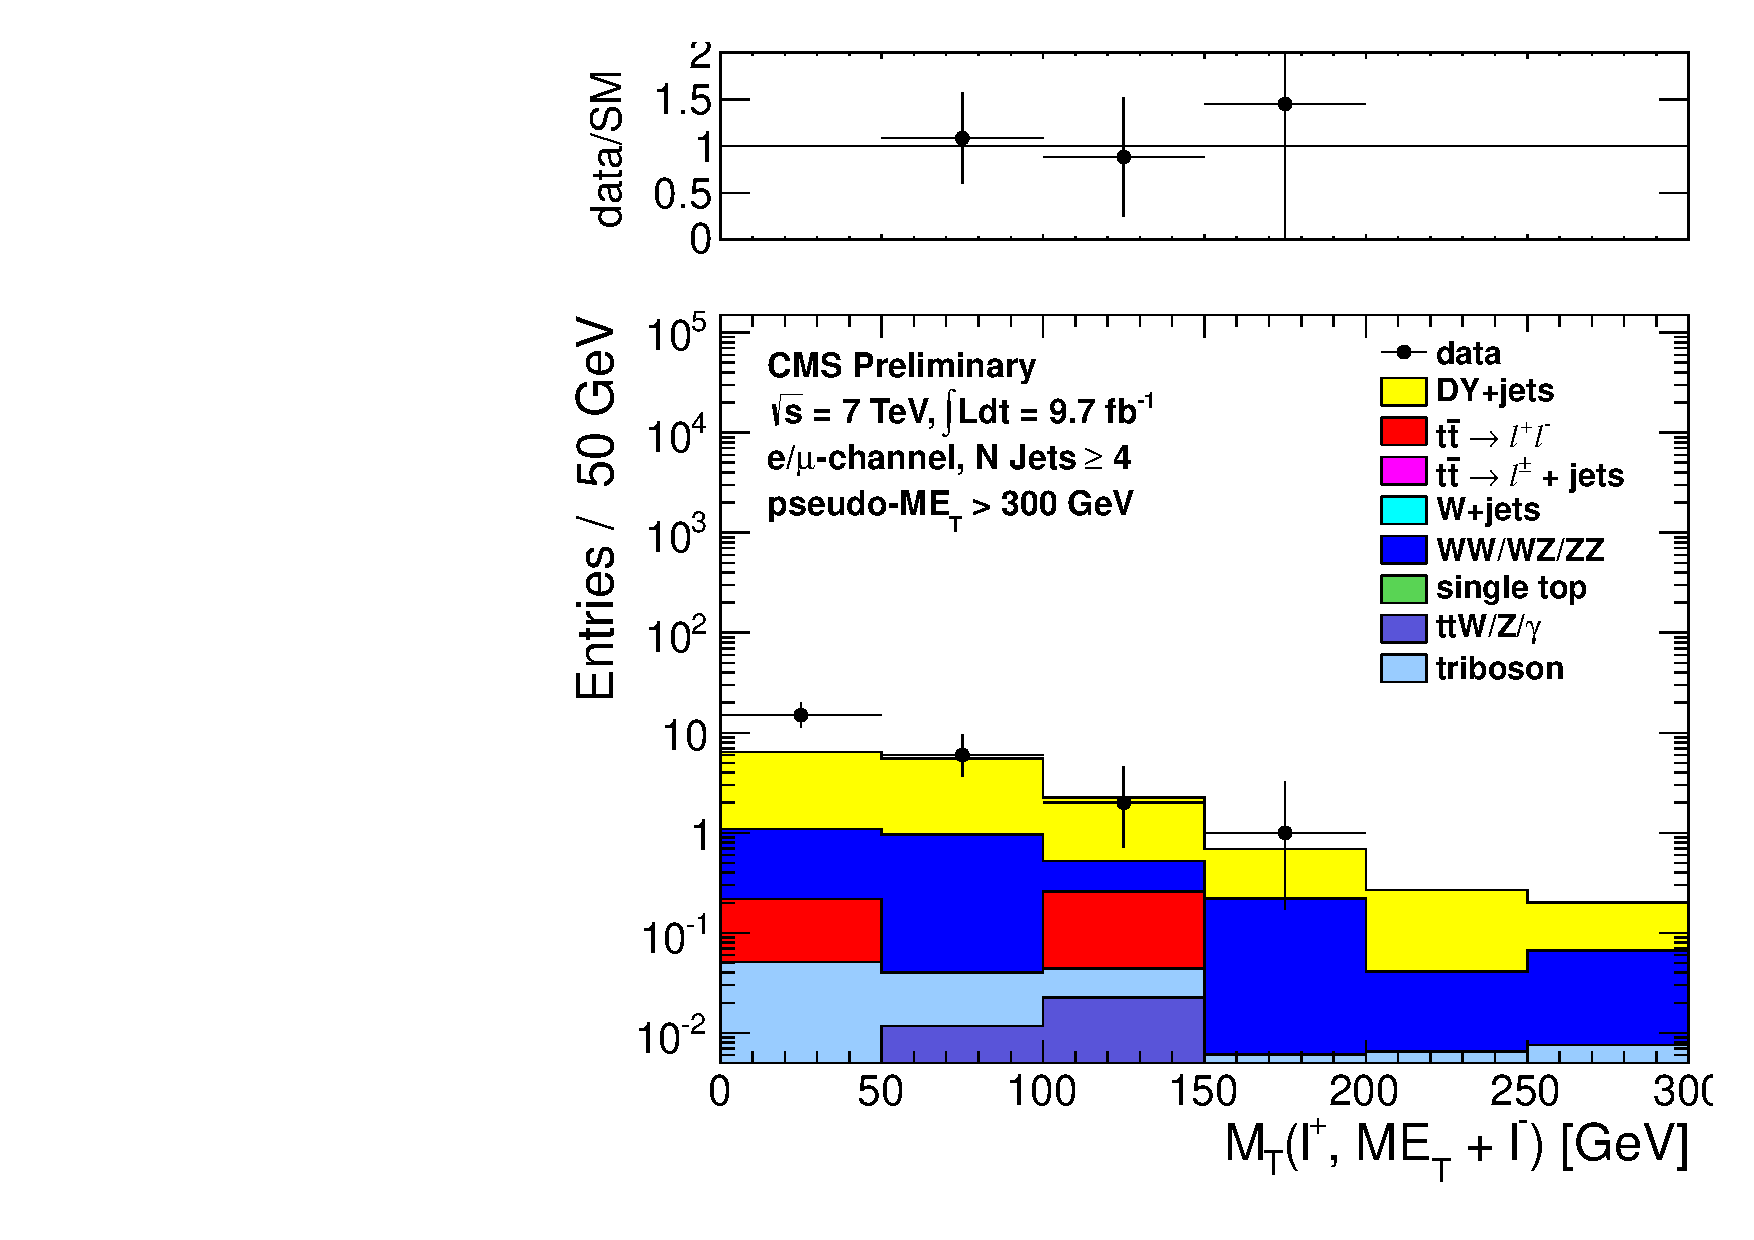
\includegraphics[width=0.5\linewidth]{plots/CR2plots/mt_lepcor_scaled_met300_nj4_emucomb.pdf}
    \caption{
      Comparison of the \mt\ distribution in data vs. MC for events
      satisfying the requirements of CR2, combining both the muon and
      electron channels. The pseudo-\met\ requirements used are
      150 GeV (top, left), 200 GeV (top, right), 250 GeV (bottom,
      left) and 300 GeV (bottom, right).
\label{fig:cr2mtrest} 
}  
      \end{center}
\end{figure}
\clearpage
